\subsection{Resources}

\subsubsection{Manpower}
The TUBULAR team is categorized into divisions as summarized in Table \ref{tab:divisions-members}:

\begin{table}[H]
\centering
\resizebox{\textwidth}{!}{%
\begin{tabular}{|l|l|l|l|l|}
\hline
\textbf{Management} & \textbf{Scientific}    & \textbf{Mechanical} & \textbf{Electrical} & \textbf{Software}          \\ \hline
Georges Labrèche*    & Kyriaki Blazaki*        & Pau Molas Roca*      & Hamad Siddiqi*       & Muhammad Ansyar Rafi Putra* \\ \hline
                    & Nuria Agues Paszkowsky & Jordi Coll Ortega   & Natalie Lawton      & Gustav Dyrssen             \\ \hline
                    &                        &                     & Ivan Zankov         &                            \\ \hline
\end{tabular}%
}
\caption{Project Divisions and Members (Asterisks Denote Division Leaders)}
\label{tab:divisions-members}
\end{table}
\raggedbottom

The experience of TUBULAR team members are listed in Table \ref{tab:team-member-experience}:

% Please add the following required packages to your document preamble:
% \usepackage{graphicx}
\begin{table}[H]
\centering
\begin{tabular}{|l|m{11cm}|}
\hline
\textbf{Team Member} & \textbf{Project Related Experience} \\ \hline
Georges L. J. Labrèche & BSc in Software Engineering with experience in technical leadership and project management in software development.\\ \hline
Nuria Agues Paszkowsky & BSc in Aerospace Engineering.\\ \hline
Kyriaki Blazaki & BSc in Physics. \\ \hline
Emily Chen & MSc in Space Engineering (4th Year). \\ \hline
Jordi Coll Ortega &  BSc in Aerospace Vehicle Engineering. \\ \hline
Gustav Dyrssen &  MSc in Space Engineering (4th Year).\\ \hline
Erik Fagerström & MSc in Space Engineering (4th Year). \\ \hline
Natalie Lawton & MEng in Aerospace Engineering. Previous experience in UAV avionic systems and emissions measurement techniques. \\ \hline
Muhammad Ansyar Rafi Putra & BSc in Aerospace Engineering. \\ \hline
Pau Molas Roca & BSc in Aerospace Technology Engineering, Mechanical experience. \\ \hline
Emil Nordqvist & MSc in Space Engineering (4th Year). \\ \hline
Hamad Siddiqi & BSc in Electrical Engineering with experience in telecommunication industry and electronics.  \\ \hline
Ivan Zankov & BEng in Mechanical Engineering.\\ \hline
\end{tabular}
\caption{Project Related Experience of Team Members}
\label{tab:team-member-experience}
\end{table}
\raggedbottom

The initial projected effort to be contributed by each team member is of an average of 1.5 hour per person per day corresponding to a team total of 15 hours per day. Taking into account all team members, the efforts projected to be allocated to each stages of the project is summarized in Table \ref{tab:effort-allocation-stages}:

\begin{table}[H]
\centering
\begin{tabular}{lcc|c|c|c|c|}
\hline
\multicolumn{1}{|c|}{\multirow{2}{*}{\textbf{Stage}}} & \multicolumn{1}{c|}{\multirow{2}{*}{\textbf{\begin{tabular}[c]{@{}c@{}}Start\\ Date\end{tabular}}}} & \multirow{2}{*}{\textbf{\begin{tabular}[c]{@{}c@{}}End\\ Date\end{tabular}}} & \multirow{2}{*}{\textbf{\begin{tabular}[c]{@{}c@{}}Duration\\ (days)\end{tabular}}} & \multicolumn{3}{c|}{\textbf{Effort (hours)}} \\ \cline{5-7} 
\multicolumn{1}{|c|}{} & \multicolumn{1}{c|}{} &  &  & \textbf{Capacity} & \textbf{Actual} & \multicolumn{1}{l|}{\textbf{Diff. (\%)}} \\ \hline
\multicolumn{1}{|l|}{Preliminary Design} & \multicolumn{1}{c|}{08/01} & 11/02 & 35 & 525 & 708 & +29.68 \\ \hline
\multicolumn{1}{|l|}{Critical Design} & \multicolumn{1}{c|}{12/02} & 03/06 & 112 & 1,680 & 2,649 & +57.66 \\ \hline
\multicolumn{1}{|l|}{Experiment Building and Testing} & \multicolumn{1}{c|}{04/06} & 16/09 & 105 & 2,048 & 1,943 & -5.40 \\ \hline
\multicolumn{1}{|l|}{Final Experiment Preparations} & \multicolumn{1}{c|}{17/09} & 11/10 & 25 & 488 & 571 & +17.00 \\ \hline
\multicolumn{1}{|l|}{Launch Campaign} & \multicolumn{1}{c|}{12/10} & 22/10 & 10 & 390 & 777 & +99.23 \\ \hline
\multicolumn{1}{|l|}{Data Analysis and Reporting} & \multicolumn{1}{c|}{23/10} & 30/01 & 69 & 1,346 & 245 & -81.78 \\ \hline
\multicolumn{1}{r}{\textbf{}} & \multicolumn{1}{l}{} & \multicolumn{1}{r|}{\textbf{Total:}} & \textbf{356} & \textbf{7,989} & \textit{6939} & \textit{-13.14} \\ \cline{4-7} 
\end{tabular}
\caption{Project Effort Allocation per Project Stages.}
\label{tab:effort-allocation-stages}
\end{table}

All TUBULAR team members are based in Kiruna, Sweden, just 40 kilometers from Esrange Space Center. Furthermore, all team members are enrolled in LTU Master programmes in Kiruna and thus expected to remain in Kiruna during the entire project period. Special attention will have to be made for planning during the summer period where many team members are expected to travel abroad. An initial timeline of team member availability  until January 2019 is available in Appendix \ref{sec:appD}. A significant risk can be observed during the summer months from June to August where most members will only be partially and some completely unavailable. Team member availability and work commitments over the summer still need to be negotiated and finalized across team members in order to reduce incurred risks to the project. Furthermore, the Project Manager role will have to be assigned to another team member due to extended unavailability and partial availability.

As part of their respective Master programmes, all TUBULAR team members are enrolled in a project course at LTU. The TUBULAR project acts as the course's project for all team members from which they will obtain ECTS credits. This course is supervised by Dr. Thomas Kuhn, Associate Professor at LTU.

\pagebreak
\subsubsection{Budget}
LTU will provide financial assistance for part of the hardware expenses, approximately 250 EUR per team member. This brings the total budget to 2 500 EUR thus far. However, the total cost of the project is 8 376.65 EUR\footnote{The cost of some items have been estimated due to lack of direct quotes from vendors. A total error margin of 5\% has been included in the final budget to account for possible estimation errors.}. In order to fill this budget gap, the following potential sources of funding are to be explored throughout the first stages of the project implementation:

\begin{itemize}
    \item The Swedish National Space Board, SNSB, will be reached out to during their next open call to researchers in Sweden to apply for funding for Space Research, including Earth Observation Research.
    \item The Swedish Research Council typically opens calls for \enquote{Proof of Concept Grant – Life science} as well as \enquote{Natural and Engineering Sciences} research grants to which an application will be sent to during the upcoming 2018 calls.
    \item Meteorological institutes, research initiatives, researchers, academic institutions, and institutional donors involved in climate change will be reached out to for contributions based on the interest of collaborating in the experiment.
    \item Third-party providers of required equipment, components, and materials will be approached with an opportunity for these providers to sponsor the project through donation before considering the related expenses. Visibility of the experiment through the planned outreach programs will serve as a visibility incentive to encourage such contributions.
    \item A small online crowdfunding campaign will be organized that will primarily target contributions from the team members' first and second degree contacts.
\end{itemize}

The project budget is detailed in Table \ref{tab:budget-table}. The budget table does not include costs related to component redundancy and as such consist of the minimum cost to build the experiment. Not included in the total are components supplied by partners and potential sponsors (e.g. the CAC tube supplied by FMI). Funding from LTU covers 28\% of the total costs while it is projected that a SNSB grant will cover 31\%. The remaining costs are associated with the air sampling bags for which sponsorship will actively be sought from a manufacturer (at the time of writing, discussions with the manufacturer Restek Corporation are ongoing regarding sponsorship of air sampling bags). 

\pagebreak
%\begin{longtable}[]
{|c|l|l|}
\hline
\multicolumn{2}{|l|}{\textbf{Expenses and Revenue per Department}} & Amount (\EUR{}) \\ \hline
\multicolumn{1}{|c|}{\multirow{5}{*}{\textbf{Electronics}}} & Components\footnote{Total cost for components is based upon Table \ref{tab:electrical-components}.} (excluding valves) & 450 \\
\multicolumn{1}{|c|}{} & Valves & 2000 \\
\multicolumn{1}{|c|}{} & Shipping Costs & 100 \\
\multicolumn{1}{|c|}{} & Tools and Equipment & 200 \\ \cline{2-3} 
\multicolumn{1}{|c|}{} & \textbf{Total Electronics Cost} & 2750 \\ \hline
\multicolumn{1}{|c|}{\multirow{6}{*}{\textbf{Mechanics}}} & Components\footnote{Total cost for mechanics is based upon Table \ref{tab:mechanical-components}.} & 450 \\
\multicolumn{1}{|c|}{} & Manufacturing & TBD \\
\multicolumn{1}{|c|}{} & Testing (Structural and Thermal) & TBD \\
%\multicolumn{1}{|c|}{} & Shipping Costs & TBD \\
\cline{2-3} 
\multicolumn{1}{|c|}{} & \textbf{Total Mechanics Cost} & TBD \\ \hline
\multicolumn{1}{|c|}{} & Project Visibility (badges, merch, website, publications, etc) & 250\\
\cline{2-3} 
\multicolumn{1}{|c|}{} & \textbf{Total Outreach} & TBD \\ \hline
\multicolumn{1}{l|}{} & \textbf{Total Costs} & TBD \\ \cline{2-3} 
\caption{Preliminary Budget Table}
\label{tab:budget-table}
\end{longtable}
\raggedbottom

\begin{table}[H]
    \begin{align*}
        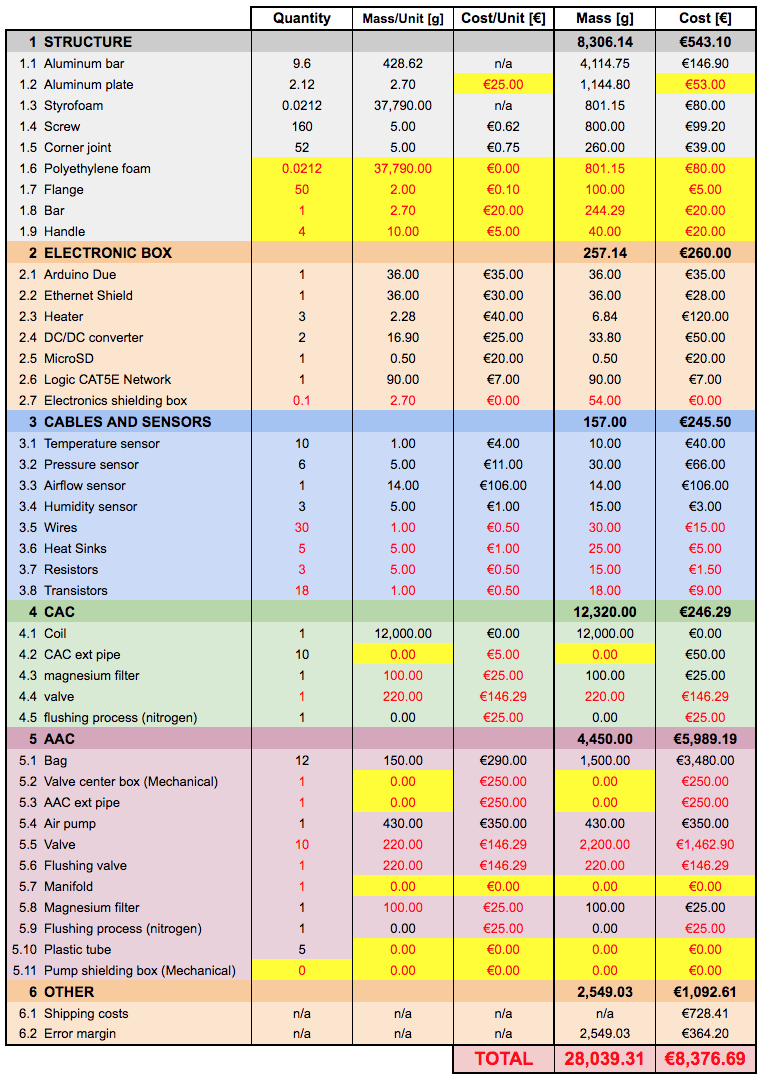
\includegraphics{3-project-planning/tables/budget-table.png}
    \end{align*}
    \caption{Project budget table. Values highlighted in yellow have yet to be determined/estimated. Number values in red have been estimated rather than determined by vendor quotes. Shipping cost is estimated at 10\% of total cost. Total cost error margin is set to 5\% of projected total cost. Total mass error margin is set to 10\% of projected total mass.}\label{tab:budget-table}
\end{table}


\subsubsection{External Support}

Partnership with the Finnish Meteorological Institute (FMI), and the Swedish Institute of Space Physics (IRF) will provide the team with technical guidance in implementing the sampling system. FMI’s experience in implementing past AirCore sample systems provide invaluable lessons learned towards conceptualizing, designing, and implementing the proposed AAC sampling system.

FMI is a key partner in the TUBULAR project, its scientific experts will advise and support the TUBULAR project by sharing knowledge, experience, and granting accessibility of equipment. As per the agreement shown in Appendix \ref{sec:appG}, FMI will provide the TUBULAR team with the AirCore stainless tube component of CAC subsystem as well as the post-flight gas analyzer. This arrangement requires careful considerations on the placement of the experiment in order to minimize hardware damage risks. These contributions will result in significant cost savings regarding equipment and component procurement.

Daily access to LTU's Space Campus in Kiruna will expose the team to scientific mentorship and expert guidance from both professors and researchers involved in the study of greenhouse gases and climate change. Dr Uwe Raffalski, Swedish institute of Space physics (IRF), Associate professor (Docent) is one of many researchers involved in climate study who is mentoring the team.